\documentclass[11pt,a4paper]{article}

\usepackage[a4paper,margin=2.4cm]{geometry}
\usepackage[T1]{fontenc}
\usepackage[utf8]{inputenc}
\usepackage{lmodern}
\usepackage{amsmath,amssymb}
\usepackage{booktabs}
\usepackage{longtable}
\usepackage{graphicx}
\usepackage{hyperref}
\usepackage{enumitem}
\usepackage{xcolor}

\hypersetup{
  colorlinks=true,
  linkcolor=blue,
  urlcolor=blue,
  pdftitle={HADROS User Manual},
  pdfauthor={HADROS}
}

\setlist[itemize]{noitemsep,topsep=3pt}
\setlist[enumerate]{noitemsep,topsep=3pt}
\emergencystretch=2em

\title{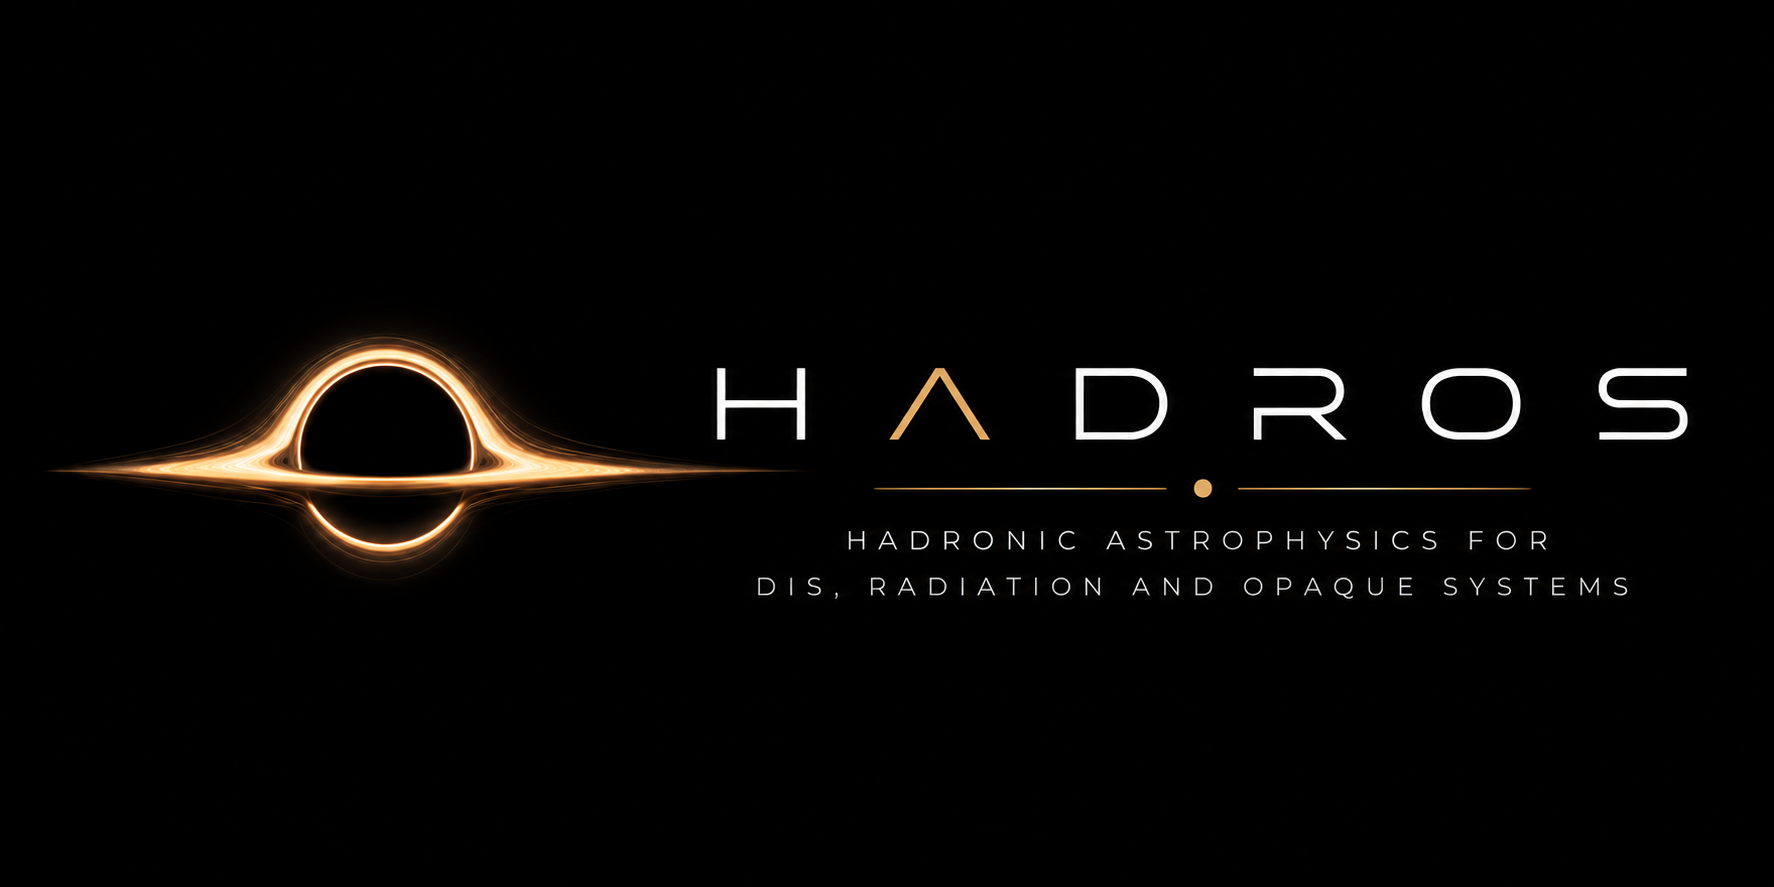
\includegraphics[width=0.48\textwidth]{../assets/Hadros_logo.png}\\[1em]
HADROS User Manual\\
\large High-energy Astrophysical DIS Radiation and Observation Simulator}
\author{HADROS}
\date{\today}

\begin{document}

\maketitle
\tableofcontents
\newpage

\section{Overview}

HADROS combines Kerr ray tracing, semi-analytic astrophysical backgrounds, UHE
neutrino DIS opacity, phenomenological source and spectral prescriptions,
diagnostic MeV neutrino post-processing, ParaView export, and a static dashboard
for organizing plots.

\begin{figure}[h]
\centering
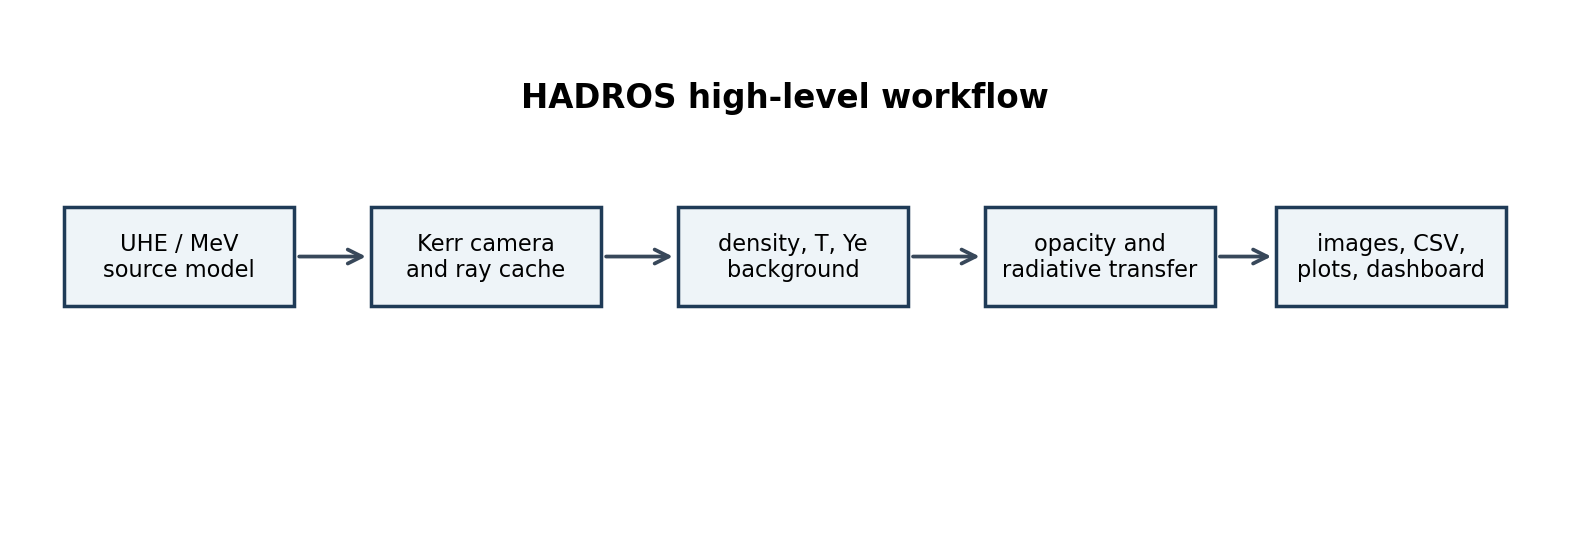
\includegraphics[width=0.95\textwidth]{figures/manual_pipeline_scheme.png}
\caption{High-level HADROS workflow.}
\end{figure}

At a high level the pipeline is
\[
\mathrm{source}\rightarrow \mathrm{Kerr\ rays}\rightarrow
\mathrm{background}\rightarrow \mathrm{opacity/transfer}\rightarrow
\mathrm{images\ and\ diagnostics}.
\]

HADROS does not perform hydrodynamic evolution. It is not full neutrino
radiation hydrodynamics, not a calibrated collapsar simulation, and not a
complete PDF-uncertainty package. The current backgrounds are semi-analytic
density morphologies, the UHE sources are phenomenological prescriptions, and
the MeV luminosities are diagnostic proxies.

\section{Physical Theories}

\subsection{Kerr Ray Tracing}

The spacetime around a rotating black hole is modeled with the Kerr metric. The
main physical parameters are the black-hole mass \texttt{MBH\_MSUN} and the
dimensionless spin \texttt{ASPIN}. The observer is placed at a large radius
\texttt{CAM\_R\_OBS\_RG} and inclination \texttt{CAM\_THETA\_DEG}. The camera
launches rays backward through the Kerr geometry and stores geodesics in a
cache.

For neutrinos in the UHE range, the rest mass is negligible compared with the
energy, so the propagation is approximated by null geodesics:
\[
ds^2 = 0.
\]
The ray path is therefore controlled by the Kerr geometry. The energy
dependence in UHE images mostly enters through opacity, $\sigma_{\nu N}(E)$,
not through chromatic lensing.

\subsection{Semi-analytic Density Backgrounds}

The matter field is a controlled semi-analytic background, not a hydrodynamic
solution. Available density profiles include \texttt{gaussian},
\texttt{powerlaw}, funnel variants, envelope variants, and
\texttt{collapsar\_ndaf\_like}.

Every profile applies an explicit density floor:
\[
\rho = \max(\rho_{\rm raw},\rho_{\rm floor}).
\]

\begin{longtable}{p{0.25\textwidth}p{0.22\textwidth}p{0.43\textwidth}}
\toprule
Regime & Purpose & Interpretation and limitation\\
\midrule
\texttt{fiducial\_uhe\_default} & UHE baseline & Low-density transparent test background; not a collapsar disk.\\
\texttt{fiducial\_mev\_density} & MeV baseline & Around $10^9$--$10^{10}$ g cm$^{-3}$ in audits; weakly cooled torus with expected low luminosity.\\
\texttt{collapsar\_ndaf\_like} & high-density preset & Significant regions near $10^{10}$--$10^{12}$ g cm$^{-3}$; semi-analytic NDAF/collapsar-like regime, not hydrodynamics.\\
\bottomrule
\end{longtable}

\subsection{UHE Neutrino DIS Opacity}

The UHE optical depth is computed from the baryon column along a ray:
\[
\tau_{\rm DIS}(E)=\int n_b(s)\,\sigma_{\nu N}(E)\,ds,
\qquad
P_{\rm surv}(E)=\exp[-\tau_{\rm DIS}(E)].
\]

HADROS currently compares \texttt{GBW}, \texttt{IIM},
\texttt{CTW\_reference}, and \texttt{literature\_powerlaw\_scale}.
\texttt{CTW\_reference} is the central $\nu N$ charged-current table from
Connolly, Thorne \& Waters, Phys. Rev. D 83, 113009, Table I. It does not
include neutral-current interactions, antineutrino tables, regeneration, or PDF
uncertainty bands.

\begin{figure}[h]
\centering
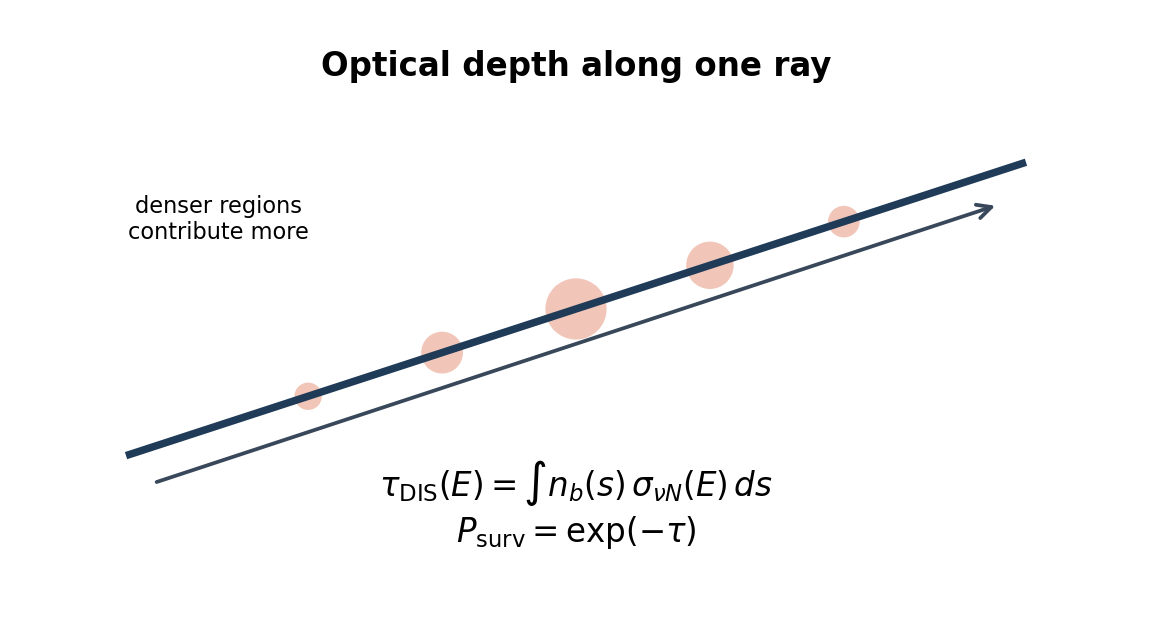
\includegraphics[width=0.75\textwidth]{figures/manual_tau_concept.png}
\caption{Optical depth and survival probability along a ray.}
\end{figure}

\subsection{UHE Source Morphologies}

The UHE emissivity is separated into a source morphology and a spectral model.
Implemented source morphologies are \texttt{inner\_ring},
\texttt{funnel\_wall}, \texttt{jet\_base}, \texttt{shock\_layer}, and
\texttt{density\_weighted}. These are phenomenological source morphologies, not
first-principles particle-acceleration simulations.

\subsection{UHE Spectral Models}

The spectral interface currently supports \texttt{monochromatic},
\texttt{powerlaw}, and \texttt{powerlaw\_cutoff}. The power-law spectrum is
\[
\frac{dN}{dE}\propto E^{-\gamma},
\]
and the cutoff model is
\[
\frac{dN}{dE}\propto E^{-\gamma}\exp(-E/E_{\rm cut}).
\]
Energy-band composite images use false colors: blue for low-energy UHE,
green for intermediate-energy UHE, and red for high-energy UHE.

\subsection{Optical-depth Surfaces}

HADROS can extract diagnostic opacity surfaces such as $\tau=2/3$, $\tau=1$,
and $\tau=3$. These surfaces are properties of the medium, geometry, energy,
and DIS cross section. They do not depend on the UHE source morphology. The
current extraction is axisymmetric and returns $r_\tau(\theta)$.

\subsection{Thermal MeV Neutrino Module}

The MeV module is separate from UHE/DIS. It is a diagnostic local emissivity and
radiative-transfer model, not a calibrated absolute luminosity prediction.
Implemented channels include URCA-like processes,
\[
e^-+p\rightarrow n+\nu_e,\qquad
e^+ + n\rightarrow p+\bar{\nu}_e,
\]
pair annihilation,
\[
e^-+e^+\rightarrow \nu+\bar{\nu},
\]
and nucleon-nucleon bremsstrahlung,
\[
N+N\rightarrow N+N+\nu+\bar{\nu}.
\]
The local transfer equation is
\[
\frac{dI}{ds}=j-\alpha I.
\]
CPU MeV is the canonical physical reference implementation. CUDA MeV remains
legacy/toy until it is ported and validated.

\begin{figure}[h]
\centering
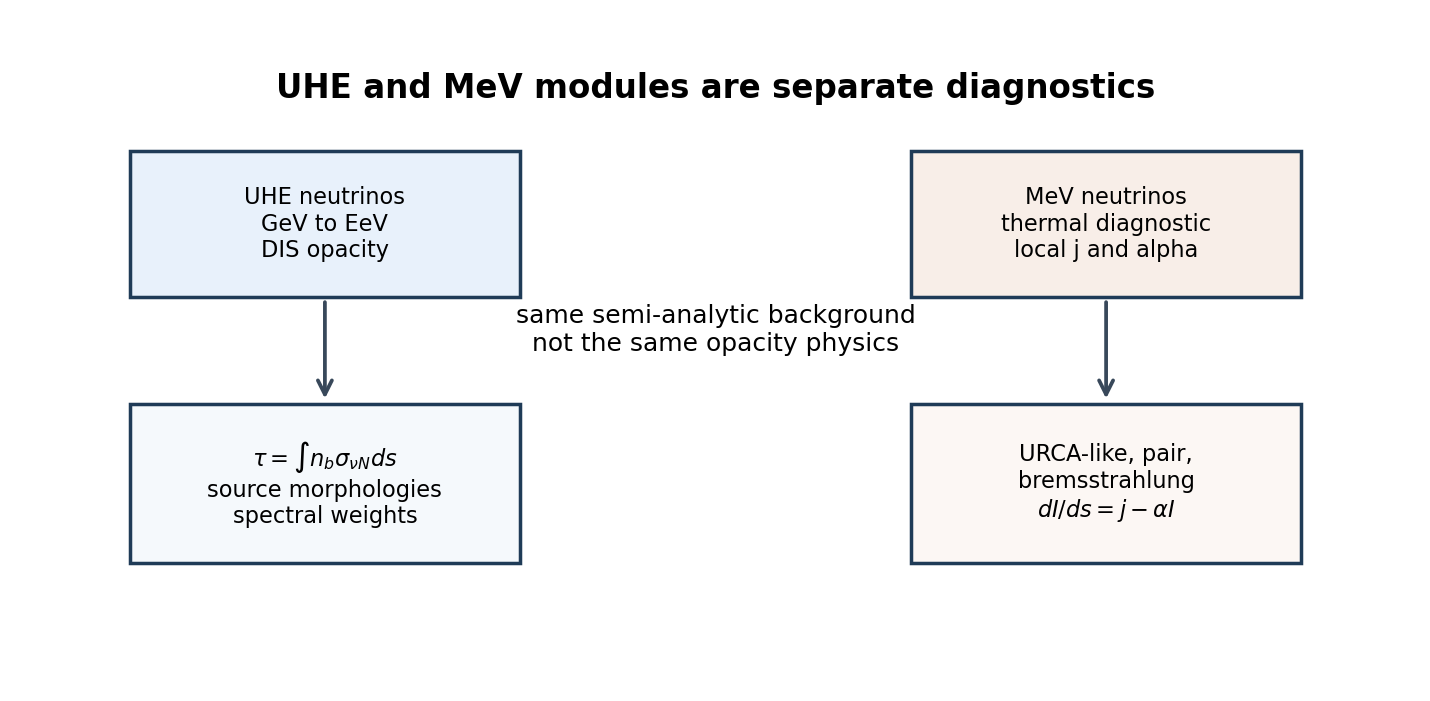
\includegraphics[width=0.86\textwidth]{figures/manual_uhe_vs_mev_physics.png}
\caption{UHE and MeV modules are separate diagnostics.}
\end{figure}

\subsection{MeV Diagnostic Upgrades}

The MeV workflow includes temperature profiles, electron-fraction profiles,
Fermi-Dirac-like spectral integration, MeV neutrinosphere extraction at
$\tau_{\rm MeV}=2/3$, electron-degeneracy diagnostics, opacity-component
decomposition, and luminosity-proxy audits.

\subsection{ParaView and 3D Visualization}

The ParaView export samples the current axisymmetric semi-analytic model onto a
3D Cartesian grid. It is not a fully 3D hydrodynamical simulation and does not
export a fake local optical-depth field.

\section{Main Makefile Commands}

\subsection{Safe Build and Validation}

\begin{verbatim}
make
make build NTHREADS=2
make validate_small NTHREADS=2
make validate_small_cuda NTHREADS=2 \
  NVCC=/home/rafael/micromamba/envs/dis/bin/nvcc \
  PYTHON=/home/rafael/micromamba/envs/dis/bin/python
make validate_medium_cuda NTHREADS=2 \
  NVCC=/home/rafael/micromamba/envs/dis/bin/nvcc \
  PYTHON=/home/rafael/micromamba/envs/dis/bin/python
\end{verbatim}

\subsection{Running Images}

\begin{verbatim}
make image-from-cache ENU=1e11 DENSITY_PROFILE=gaussian NTHREADS=2
make image-from-cache SPECTRAL_MODEL=powerlaw \
  SPECTRAL_GAMMA=2.0 SPECTRAL_E_MIN_GEV=1e5 \
  SPECTRAL_E_MAX_GEV=1e12 SPECTRAL_N_BINS=8 NTHREADS=2
make plot_multiband_image PYTHON=python3
make image-from-cache MEV_MODEL=physical MEV_FLAVOR=anti_nu_e NTHREADS=2
make mev_multiband_image NTHREADS=2 PYTHON=python3
\end{verbatim}

\subsection{Robustness, DIS, Opacity, and MeV Diagnostics}

\begin{verbatim}
make robustness_scans NTHREADS=2 PYTHON=python3
make validate_dis_models NTHREADS=2 PYTHON=python3
make opacity_surfaces TAU_SURFACE_VALUE=1.0 PYTHON=python3
make validate_mev_physics PYTHON=python3
make mev_neutrinosphere PYTHON=python3
make mev_luminosity PYTHON=python3
make audit_mev_luminosity PYTHON=python3
make audit_torus_regime PYTHON=python3
make audit_collapsar_ndaf_like PYTHON=python3
\end{verbatim}

\subsection{ParaView and Dashboard}

\begin{verbatim}
make paraview_fields \
  DENSITY_PROFILE=powerlaw_funnel_envelope \
  SOURCE_MODEL=funnel_wall \
  PARAVIEW_NX=64 PARAVIEW_NY=64 PARAVIEW_NZ=64 \
  PARAVIEW_BOX_RG=80 NTHREADS=4

make dashboard PYTHON=python3
\end{verbatim}

Open \texttt{dashboard/index.html} in a browser. The dashboard indexes existing
plots and output products; it does not run simulations.

\subsection{Thread Control}

Use explicit limits:
\begin{verbatim}
make -j2 build
make validate_small NTHREADS=2
make run_production NTHREADS=4
\end{verbatim}
The default \texttt{make} target prints help and does not launch a production
simulation.

\section{Outputs and Directory Map}

\begin{figure}[h]
\centering
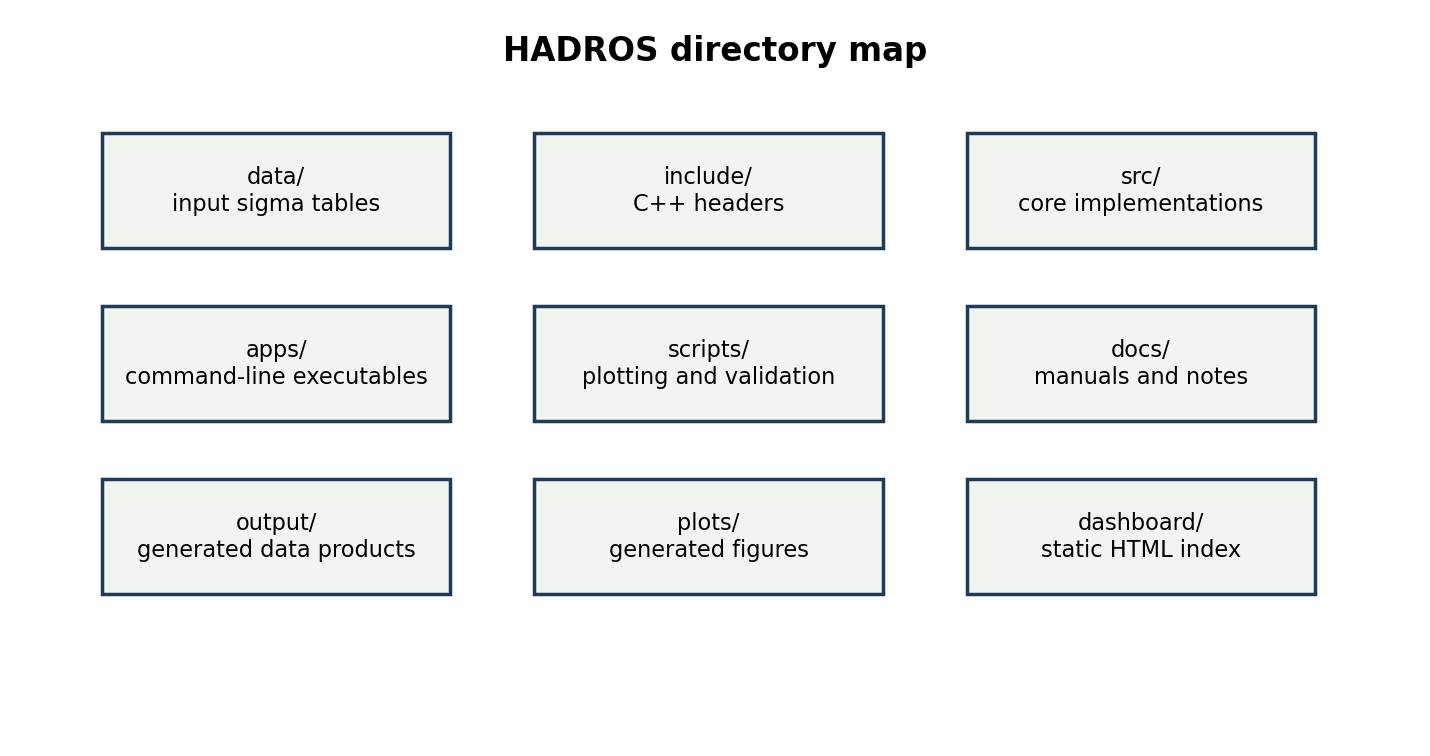
\includegraphics[width=0.86\textwidth]{figures/manual_directory_map.png}
\caption{Main HADROS directories.}
\end{figure}

\begin{itemize}
\item \texttt{data/}: input data tables, especially DIS sigma tables.
\item \texttt{include/}: C++ headers.
\item \texttt{src/}: core implementations.
\item \texttt{apps/}: command-line applications.
\item \texttt{scripts/}: plotting, validation, and audit scripts.
\item \texttt{docs/}: manuals and scientific notes.
\item \texttt{plots/}: generated figures.
\item \texttt{output/}: generated tables, images, ray caches, and reports.
\item \texttt{dashboard/}: static HTML dashboard.
\end{itemize}

\section{Program Workflow}

The internal workflow is:
\begin{enumerate}
\item choose a physical setup;
\item generate or load a Kerr ray cache;
\item evaluate the local background along each ray;
\item compute local UHE and/or MeV emissivity;
\item compute opacity;
\item integrate radiative transfer along rays;
\item write data tables;
\item generate plots;
\item index products in the dashboard.
\end{enumerate}

\section{Recommended Workflows for Students}

Beginner dashboard:
\begin{verbatim}
make dashboard PYTHON=python3
\end{verbatim}

Beginner validation:
\begin{verbatim}
make validate_small NTHREADS=2 PYTHON=python3
\end{verbatim}

Intermediate DIS comparison:
\begin{verbatim}
make validate_dis_models NTHREADS=2 PYTHON=python3
\end{verbatim}

Intermediate MeV diagnostics:
\begin{verbatim}
make validate_mev_physics PYTHON=python3
\end{verbatim}

Advanced collapsar/NDAF-like comparison:
\begin{verbatim}
make audit_collapsar_ndaf_like PYTHON=python3
\end{verbatim}

Advanced ParaView export:
\begin{verbatim}
make paraview_fields DENSITY_PROFILE=collapsar_ndaf_like NTHREADS=4
\end{verbatim}

\section{Scientific Limitations}

\begin{itemize}
\item Backgrounds are semi-analytic, not hydrodynamic evolutions.
\item HADROS does not solve full neutrino radiation hydrodynamics.
\item MeV luminosities are proxy/diagnostic quantities.
\item CUDA MeV remains legacy/toy and is not equivalent to CPU physical MeV.
\item \texttt{CTW\_reference} is central charged-current $\nu N$ only.
\item UHE neutral-current interactions and regeneration are not yet included.
\item There is no true 3D hydrodynamic background yet.
\end{itemize}

\section{Troubleshooting}

If \texttt{make} seems to run too long, stop the process and use a validation
target such as \texttt{validate\_small}. If CPU usage is too high, pass
\texttt{NTHREADS=2} or \texttt{NTHREADS=4}, and use limited make parallelism
such as \texttt{make -j2 build}. If CUDA is not found, check \texttt{which
nvcc}, \texttt{nvcc --version}, and \texttt{nvidia-smi}. If plots are missing,
regenerate the relevant plot target and rebuild the dashboard. If stale caches
are suspected after a crash, see \texttt{README\_RECOVERY\_20260609.md}.

\section{Glossary}

\begin{description}
\item[DIS] Deep inelastic scattering, the high-energy neutrino-nucleon
interaction used for UHE opacity.
\item[UHE] Ultra-high energy, here referring to GeV-to-EeV scale neutrinos.
\item[MeV] Thermal neutrino energy scale used in the diagnostic module.
\item[Optical depth] Dimensionless attenuation measure, $\tau$.
\item[Survival probability] $P_{\rm surv}=\exp(-\tau)$.
\item[Neutrinosphere] Diagnostic surface where optical depth reaches a chosen
value, often $\tau=2/3$.
\item[Kerr metric] Spacetime geometry around a rotating black hole.
\item[NDAF] Neutrino-dominated accretion flow.
\item[Collapsar] Massive-star collapse scenario that can form a black hole and
dense accretion environment.
\item[CTW] Connolly, Thorne \& Waters reference cross-section table.
\item[GBW] Golec-Biernat-Wusthoff saturation-inspired DIS model.
\item[IIM] Iancu-Itakura-Munier saturation-inspired DIS model.
\end{description}

\end{document}
